\documentclass[11pt]{article}

\usepackage[a4paper,margin=2.4cm]{geometry}
\usepackage{amsmath,amssymb}
\usepackage{graphicx}
\usepackage{booktabs}
\usepackage{array}
\usepackage{enumitem}
\usepackage{caption}
\usepackage[british]{babel}
\usepackage{csquotes}
\usepackage[style=apa,backend=biber]{biblatex}
\addbibresource{references.bib}
\usepackage[hidelinks]{hyperref}

\graphicspath{{figures/}}
\captionsetup{font=small,labelfont=bf}
\setlist{nosep,leftmargin=1.4em}

\newcommand{\Lc}{\mathcal{L}}
\newcommand{\Hyp}{\mathcal{H}}

\title{\vspace{-1.5em}\textbf{Studying Loss Functions and the Training Criterion}\\[0.3em]
\large A2 Project Report and Implementation Log}
\author{Daniel James Martirosov\\ Student ID 24948933\\[0.2em]
\normalsize Advanced Data Analytics Algorithms, Machine Learning\\ \normalsize 2026}
\date{}

\begin{document}
\maketitle
\vspace{-2.2em}

\begin{center}
\small
\textbf{Option 1: study and implement a fundamental machine learning model.}
\end{center}

\section*{Link to Implementation}

The complete, self-contained notebook is archived publicly at:

\begin{itemize}
  \item GitHub: \url{https://github.com/MathgeniusTB2/a2-mlp-from-scratch/blob/main/a2_mlp_numpy.ipynb}
\end{itemize}

The notebook contains the whole implementation: environment setup, data downloading and
preprocessing, the model, the five training criteria and their gradients, the learning
algorithm, the cross-validation study, the per-epoch training and held-out validation learning
curves, the final test evaluation and the error analysis. It runs end to end on a stock Colab
runtime: it needs only NumPy and Matplotlib, both preinstalled, and downloads the dataset on
demand.

\section{Problem Definition}
\label{sec:problem}

\subsection{Background and Motivation}

Recognising hand-written digits was one of the first tasks used to show that a learning system
can replace a hand-written rule. The perceptron~\parencite{rosenblatt1958} could separate linearly
separable patterns, and its limits were made explicit by \textcite{minsky1969}. The decisive step was backpropagation~\parencite{rumelhart1986}, which
made a composition of affine maps and a nonlinearity trainable by gradient descent, and a
single hidden layer can approximate any continuous function~\parencite{cybenko1989,hornik1991}.
MNIST and gradient-based digit recognition followed~\parencite{lecun1998}.

The separation between the quantity a learning algorithm optimises and the quantity the task
actually rewards is not specific to this project. In statistics it is the theory of scoring
rules: a loss is \emph{proper} if it is minimised, in expectation, by the true class
probability, and \emph{strictly proper} if that minimiser is unique~\parencite{brier1950,gneiting2007}.
Cross-entropy and the Brier score (squared error on probabilities) are the canonical strictly
proper rules for a categorical target, which is why they are the natural reference points here.
Cost-sensitive learning makes the same distinction from the decision side: under asymmetric
costs the best decision is not the most probable class but the one that minimises expected
cost~\parencite{elkan2001}, and the custom expected-cost criterion in this project sits exactly at
that interface. Two further strands motivate the comparison. Label smoothing replaces the
one-hot target by a softened one; it is widely reported to help accuracy and robustness, and it
also tends to \emph{improve} calibration (reduce the expected calibration error), in the same
way as temperature scaling~\parencite{szegedy2016,muller2019}. Networks trained with plain
cross-entropy are otherwise poorly calibrated, in the sense that predicted confidence exceeds
empirical accuracy~\parencite{guo2017}. Finally, training on a surrogate that differs from the decision loss
is justified in general by consistency results for convex surrogate losses~\parencite{bartlett2006};
the study below is a small, controlled instance of that phenomenon.

Every one of those results is about the \emph{hypothesis space}. This project instead studies
the third pillar of the learning framework, the \emph{criterion}: the function that the
learning algorithm actually minimises. The criterion is not something that can be chosen
freely, because a learning algorithm can only minimise a differentiable surrogate of the
decision rule we care about. The task objective here is to be right; the training loss is
cross-entropy, a strictly proper scoring rule that minimises the KL divergence to the label
distribution. When the loss is a different function -- squared error, absolute error, or a
designed cost -- the surrogate and the objective can pull in different directions. That gap is
the object of study.

\subsection{Research Question}

The question this project asks is deliberately narrow and measurable: \emph{how does the choice
of training criterion change what the multi-layer perceptron learns, and when does minimising
the loss fail to serve the task objective?} It is answered by training the same network on five
criteria and comparing accuracy, the optimised loss, and a hand-designed task objective.

\subsection{The Task}

The task is multi-class classification of hand-written digits, the classic MNIST benchmark
~\parencite{lecun1998}. This section fixes the input and output interfaces for training and
deployment.

\paragraph{Training input.}
A batch of images. Each image is a $28\times 28$ matrix of integers in $[0,255]$
(\texttt{uint8}). Every image is normalised to $[0,1]$ by dividing by $255$, then flattened to
a real vector in $\mathbb{R}^{784}$. The label is an integer in $\{0,\dots,9\}$, encoded as a
one-hot vector in $\{0,1\}^{10}$.

\paragraph{Deployment input.}
A single image in the same format, preprocessed identically and deterministically.

\paragraph{Training output (target).}
A one-hot vector in $\{0,1\}^{10}$ giving the digit's class.

\paragraph{Deployment output.}
A probability vector $p\in[0,1]^{10}$ with $\sum_k p_k = 1$. The predicted class is
$\arg\max_k p_k$, and $p_k$ is the model's estimated probability that the input is the digit
$k$. The probability vector (not just the decision) is the output because the loss is defined
on it.

\paragraph{When the input is not well behaved.}
Most images are centred digits, but not all. Digits may be slanted, faintly inked, or touching,
and a small fraction are genuinely ambiguous even to a person. Because the same image can
plausibly be read as more than one digit, the correct output is best understood as a
distribution over classes.

\subsection{Why Machine Learning Is the Right Tool}

Three conditions hold. A pattern exists (the visual structure of a digit is consistent enough
to learn). Data is available (60\,000 training and 10\,000 test images). And the rule cannot be
written in closed form: explicit \texttt{if} statements over pixel values are hopeless, because
the relationship between intensities and the concept ``this is a seven'' is spread across
variations in slant, thickness and position.

\section{Machine Learning Approach}
\label{sec:approach}

A supervised learning system has four components~\parencite{goodfellow2016}: the data, the
hypothesis space $\Hyp$, the criterion (loss) $\Lc$, and the learning algorithm. Here $\Hyp$
and the algorithm are fixed and the criterion is the variable.

\subsection{Data and Preprocessing}

The 60\,000 training images are normalised to $[0,1]$ and flattened to $\mathbb{R}^{784}$; the
10\,000 test images are preprocessed identically. The test set is used only for the final
evaluation. Within training, 5-fold cross-validation is used to compare criteria: each fold is
the validation set in turn, so no comparison looks at the test set.

\subsection{The Model}

The hypothesis space is a two-hidden-layer MLP,
\begin{equation}
f_\theta(x) = \mathrm{softmax}\!\Big(W^{(2)}\,\tanh\big(W^{(1)}\,\tanh(W^{(0)} x + b^{(0)}) + b^{(1)}\big) + b^{(2)}\Big),
\end{equation}
with layer sizes $784\text{-}128\text{-}128\text{-}10$ (118\,282 parameters). The hidden
activation is $\tanh$, the nonlinearity used in the subject's hypothesis-family module, and the
weights are drawn from the LeCun normal distribution, $\mathcal{N}(0,1/n_{in})$, which is the
variance-preserving choice for $\tanh$ (Xavier would use $2/(n_{in}+n_{out})$; the code uses
$1/n_{in}$).

\subsection{The Training Criteria}
\label{sec:criteria}

Five criteria are compared. For a batch with predictions $\hat p$ and one-hot labels $y$:

\paragraph{Cross-entropy.}
$\Lc=-\frac1n\sum_i\sum_k y_{ik}\log\hat p_{ik}$, the negative log-likelihood. For a one-hot
target this equals the KL divergence to the label distribution, and it is a strictly proper
scoring rule.

\paragraph{Squared error.} $\Lc=\frac1n\sum_i\tfrac12\lVert \hat p_i-y_i\rVert^2$ on the softmax
outputs. Also a proper scoring rule (the Brier score), but it saturates on confident errors.

\paragraph{Absolute error.} $\Lc=\frac1n\sum_i\lVert \hat p_i-y_i\rVert_1$. For a softmax output
strictly inside $(0,1)$ and a one-hot target the sign pattern of $\hat p-y$ never changes (it is
negative at the true class and positive everywhere else), so
$\lVert \hat p-y\rVert_1=(1-\hat p_y)+\sum_{k\ne y}\hat p_k=2(1-\hat p_y)$. The loss is therefore
\emph{linear in the probability vector}, and the usual ``non-smooth at zero'' caveat does not
apply: the kink is only reached at $\hat p_y=1$ or $\hat p_k=0$, which the softmax does not
attain for finite logits. Being linear, it is not a proper scoring rule (its minimiser is a
corner, not the true probability), so it belongs to the same family as the custom expected-cost
criterion below.

\paragraph{Label smoothing.} The target is replaced by
$t_i=(1-\epsilon)y_i+\epsilon/K$ with $\epsilon=0.1$, and cross-entropy is taken against $t$.
This caps how confident the model is asked to be.

\paragraph{Custom expected cost.} A hand-designed criterion. I built a $10\times10$ reward
matrix $R$ (rows the true digit, columns the guess) where the diagonal is $10$ and visually
similar digits receive partial reward (for example $4{:}9$ gets $6$, $3{:}5$ gets $5$). Scaling
by $1/10$ puts the reward in $[0,1]$. The criterion is the expected cost of the decision,
\begin{equation}
\Lc=\frac1n\sum_i\sum_k \hat p_{ik}\,\big(1-R_{y_i,k}\big),
\label{eq:expectedcost}
\end{equation}
so a decision on a similar digit is cheaper than a decision on a dissimilar one. The full matrix
is given in Table~\ref{tab:reward}; it is symmetric, the diagonal is $10$, and the off-diagonal
entries are the coarse visual similarities (for example the $(4,9)$ and $(3,5)$ pairs are high).
Like absolute error above, this loss is linear in the probabilities, which turns out to be the
key to its behaviour (Section~\ref{sec:disc}).

\begin{table}[htbp]
\centering
\small
\caption{The hand-designed reward matrix $R$ (before the $1/10$ scaling). Rows are the true
digit, columns the predicted digit.}
\label{tab:reward}
\begin{tabular}{@{}lrrrrrrrrrr@{}}
\toprule
 & 0 & 1 & 2 & 3 & 4 & 5 & 6 & 7 & 8 & 9 \\
\midrule
0 & 10 & 0 & 1 & 1 & 0 & 1 & 2 & 0 & 1 & 1 \\
1 & 0 & 10 & 1 & 1 & 1 & 0 & 0 & 1 & 2 & 0 \\
2 & 1 & 1 & 10 & 3 & 1 & 1 & 1 & 3 & 3 & 0 \\
3 & 1 & 1 & 3 & 10 & 0 & 5 & 0 & 2 & 4 & 2 \\
4 & 0 & 1 & 1 & 0 & 10 & 1 & 2 & 2 & 1 & 6 \\
5 & 1 & 0 & 1 & 5 & 1 & 10 & 3 & 0 & 3 & 2 \\
6 & 2 & 0 & 1 & 0 & 2 & 3 & 10 & 0 & 2 & 0 \\
7 & 0 & 1 & 3 & 2 & 2 & 0 & 0 & 10 & 1 & 4 \\
8 & 1 & 2 & 3 & 4 & 1 & 3 & 2 & 1 & 10 & 2 \\
9 & 1 & 0 & 0 & 2 & 6 & 2 & 0 & 4 & 2 & 10 \\
\bottomrule
\end{tabular}
\end{table}

\subsection{Gradients and Theory-to-Code}
\label{sec:theory}

Backpropagation is derived by the chain rule, with $\delta^{(L)}=\partial\Lc/\partial z^{(L)}$
the only term that changes between criteria. Table~\ref{tab:map} maps each criterion's
mathematics to the code. The weight and bias gradients are the same for all criteria,
$\partial\Lc/\partial W^{(\ell)}=\delta^{(\ell)\top}a^{(\ell-1)}$.

\begin{table}[htbp]
\centering
\small
\caption{Each criterion, its logit gradient, and the code location.}
\label{tab:map}
\begin{tabular}{@{}p{3.5cm}p{5.4cm}p{5.2cm}@{}}
\toprule
Criterion & $\delta^{(L)}=\partial\Lc/\partial z^{(L)}$ & Code (\texttt{run}, criterion block) \\
\midrule
cross-entropy & $\frac1n(\hat p-y)$ & \texttt{d3 = (p - tgt) / n} \\
squared error & $\frac1n\,\hat p\odot\big((\hat p-y)-\sum_k(\hat p_k-y_k)\hat p_k\big)$ & \texttt{d3 = p * (r - sum(r * p)) / n} \\
absolute error & $\frac1n\,\hat p\odot\big(\mathrm{sign}(\hat p-y)-\sum_k \mathrm{sign}(\hat p_k-y_k)\hat p_k\big)$ & \texttt{d3 = p * (s - sum(s * p)) / n} \\
label smoothing & $\frac1n(\hat p-t)$ & \texttt{d3 = (p - tgt) / n} \\
expected cost & $\frac1n\,\hat p\odot\big(c-\sum_k \hat p_k c_k\big)$, $c=1-R_y$ & \texttt{d3 = p * (cost - sum(p * cost)) / n} \\
\bottomrule
\end{tabular}
\end{table}

The softmax Jacobian is what makes the non-cross-entropy gradients non-trivial: for
$\hat p=\mathrm{softmax}(z)$, the derivative of any deterministic function $g(\hat p)$ is
$\partial g/\partial z_k=\hat p_k\,(g_k-\sum_j \hat p_j g_j)$, which is exactly the form in the
table.

\subsection{Learning Algorithm}

Training is mini-batch gradient descent with Adam~\parencite{kingma2015}, implemented from scratch
with bias-corrected first and second moments. Mini-batches of 128, learning rate
$\eta=10^{-3}$, $\beta_1=0.9$, $\beta_2=0.999$, $\epsilon=10^{-8}$, 30 epochs. The same
optimiser and rate are used for every criterion, so the comparison isolates the criterion.

\subsection{Evaluation Protocol and Metrics}

The protocol separates selection from reporting. Criteria are compared by \textbf{5-fold
cross-validation} on the training set (each fold is the validation set), reported as
mean $\pm$ std across folds. Then each criterion is \textbf{refit on all 60\,000} training
images and scored \textbf{once on the official test set}, over three random seeds, reported as
mean $\pm$ std. Reported metrics are accuracy (the task decision), test cross-entropy (the quantity actually
optimised by cross-entropy and label smoothing, and reported for every criterion),
and two task-objective measures defined by the reward matrix: the mean
reward of the decision, and the mean reward over the errors (how similar the mistakes are).
A majority-class baseline sets the floor.

\paragraph{The ideal comparison.} For a classification task the ideal comparison between the
model output and the desired output is the 0--1 loss: zero for a correct decision, one
otherwise. It is used at validation and test time, where accuracy is exactly one minus the mean
0--1 loss, but it is deliberately \emph{not} used for training. Its gradient with respect to the
parameters is zero almost everywhere (the loss is piecewise constant in the output), so gradient
descent receives no signal from it; a differentiable surrogate is needed instead. Every training
criterion here is such a surrogate, and the fact that a surrogate is not the 0--1 loss is the
source of the loss--objective gaps reported below.

\section{Results}
\label{sec:results}

\subsection{Cross Validation}

Table~\ref{tab:cv} gives the 5-fold validation accuracy. Cross-entropy and label smoothing lead
($0.9786$ and $0.9782$), followed by squared error and absolute error, with the expected-cost
criterion last ($0.9720$). The largest gap is about $0.7$ points, larger than the fold-to-fold
standard deviation. Cross-entropy and label smoothing are again indistinguishable ($0.0004$
apart, standard deviations $0.0011$ and $0.0010$).

\begin{table}[htbp]
\centering
\small
\caption{5-fold cross-validation accuracy (validation folds, not the test set).}
\label{tab:cv}
\begin{tabular}{@{}lr@{}}
\toprule
Criterion & Validation accuracy (mean $\pm$ std) \\
\midrule
cross-entropy & $0.9786 \pm 0.0011$ \\
label smoothing & $0.9782 \pm 0.0010$ \\
squared error & $0.9756 \pm 0.0020$ \\
absolute error & $0.9730 \pm 0.0018$ \\
expected cost (mine) & $0.9720 \pm 0.0022$ \\
\bottomrule
\end{tabular}
\end{table}

\begin{figure}[htbp]
\centering
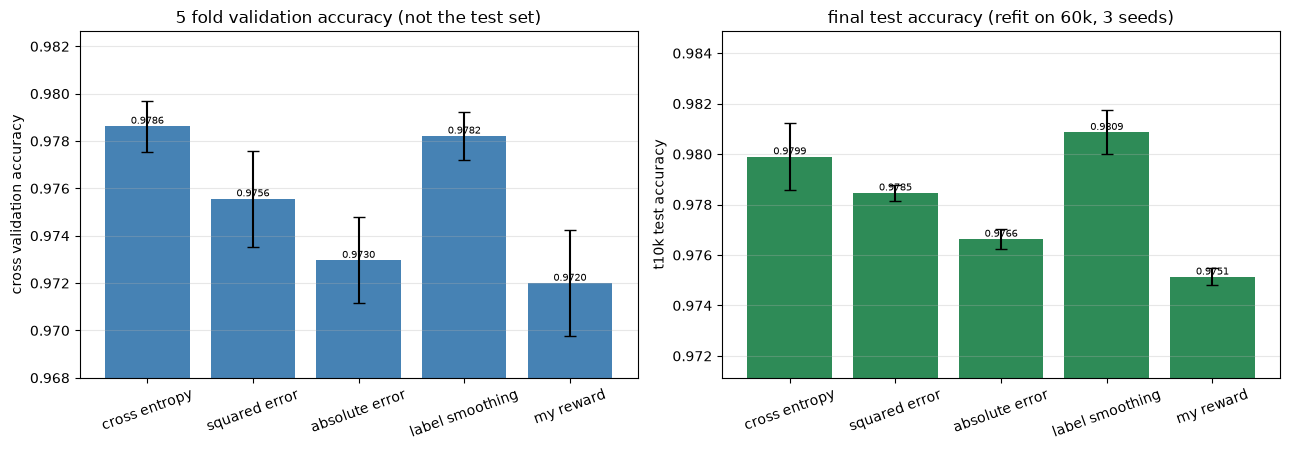
\includegraphics[width=0.9\textwidth]{fig_criterion_comparison.png}
\caption{Cross-validation accuracy (left) and final test accuracy (right).}
\label{fig:comp}
\end{figure}

\subsection{Learning Curves}
\label{sec:curves}

Figure~\ref{fig:lc} reports, for the first validation fold, the training cross-entropy (left),
the held-out validation cross-entropy (middle) and the held-out validation accuracy (right),
per epoch. Both loss panels use the \emph{same} metric, cross-entropy, for every criterion, so
the curves are directly comparable. The training cross-entropy falls steadily while the
validation cross-entropy falls and then flattens or rises, so a gap opens between them: ordinary
overfitting at this capacity and epoch count. Two caveats follow. First, the validation accuracy
is still creeping up slightly at epoch 30, so the models are not fully converged. Second, the
validation cross-entropy for cross-entropy rises after about epoch 10 while that for squared
error keeps falling, so the test-cross-entropy ranking partly reflects \emph{different
overfitting}, not only the criterion; no early stopping is used. The validation curve is
computed on a \emph{held-out} fold; it is never the training set. Training and validating on the
same data would make the curve measure only how well the model fits, not how well it
generalises.

\begin{figure}[htbp]
\centering
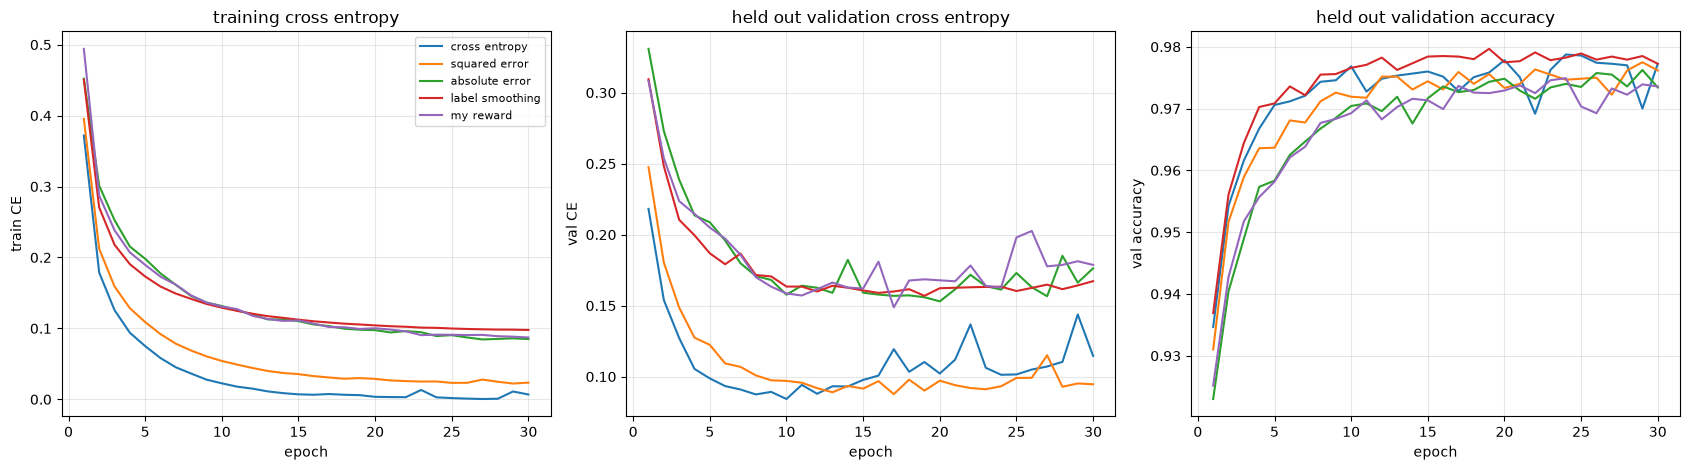
\includegraphics[width=0.98\textwidth]{fig_learning_curves.png}
\caption{Training cross-entropy, held-out validation cross-entropy and held-out validation
accuracy by epoch, on validation fold 0.}
\label{fig:lc}
\end{figure}

\subsection{Final Test Set}

Table~\ref{tab:test} gives the final test numbers, each refit on all 60\,000 images over three
seeds and reported as mean $\pm$ std. Two differences are real and two are not. \emph{Real:} the
expected-cost criterion is last on accuracy ($0.9751$), and squared error has the lowest test
cross-entropy ($0.0826$). \emph{Not real:} label smoothing and cross-entropy differ by $0.0010$
in accuracy with standard deviations of $0.0009$ and $0.0013$, so they are not distinguishable,
and the reward-over-errors gap between them ($0.2669\pm0.0080$ against $0.2660\pm0.0036$) is
entirely within seed noise. The mean-reward column also adds nothing: its ranking is identical
to the accuracy ranking, so on this task it is a restatement of accuracy rather than an
independent objective.

\begin{table}[htbp]
\centering
\small
\caption{Final test (t10k) metrics, refit on 60\,000 images, mean over three seeds.}
\label{tab:test}
\begin{tabular}{@{}lrrrr@{}}
\toprule
Criterion & Accuracy & Test CE & Mean reward & Reward over errors \\
\midrule
label smoothing & $0.9809 \pm 0.0009$ & $0.1558 \pm 0.0018$ & $0.9860 \pm 0.0006$ & $0.2660 \pm 0.0036$ \\
cross-entropy & $0.9799 \pm 0.0013$ & $0.0927 \pm 0.0026$ & $0.9853 \pm 0.0009$ & $0.2669 \pm 0.0080$ \\
squared error & $0.9785 \pm 0.0003$ & $\mathbf{0.0826 \pm 0.0007}$ & $0.9841 \pm 0.0001$ & $0.2598 \pm 0.0055$ \\
absolute error & $0.9766 \pm 0.0004$ & $0.1577 \pm 0.0027$ & $0.9827 \pm 0.0003$ & $0.2589 \pm 0.0013$ \\
expected cost (mine) & $0.9751 \pm 0.0003$ & $0.1683 \pm 0.0020$ & $0.9816 \pm 0.0002$ & $0.2598 \pm 0.0045$ \\
\midrule
majority baseline & 0.1135 & -- & -- & -- \\
\bottomrule
\end{tabular}
\end{table}

\begin{figure}[htbp]
\centering
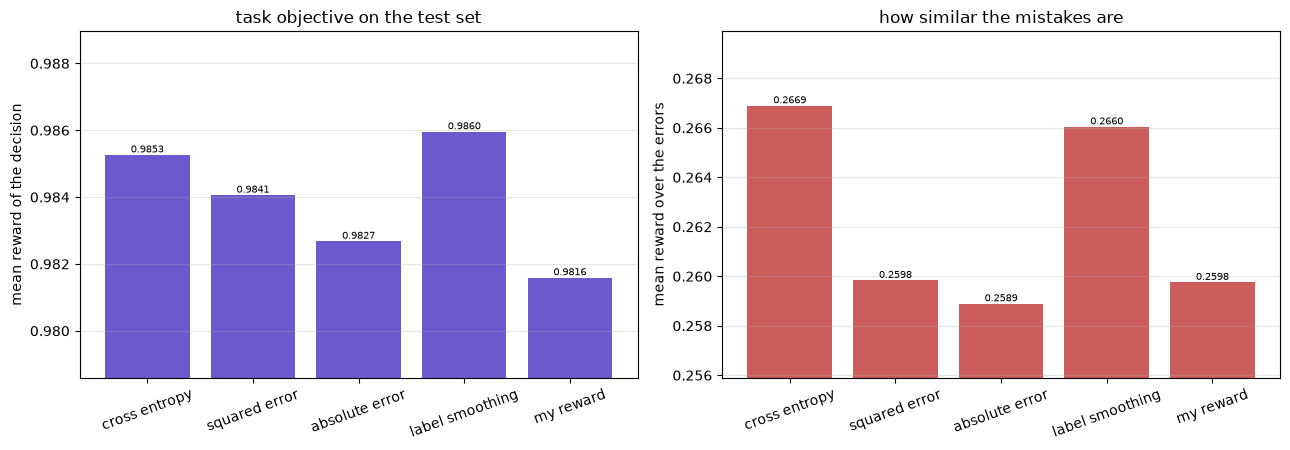
\includegraphics[width=0.9\textwidth]{fig_task_objective.png}
\caption{Task objective on the test set: mean reward of the decision (left) and mean reward
over the errors (right). Cross-entropy and squared error, the two strictly proper rules, cluster
together; the custom expected-cost criterion does not improve on them.}
\label{fig:objective}
\end{figure}

\subsection{Where the Mistakes Land}

Figure~\ref{fig:cm} shows the seed-averaged confusion matrices for cross-entropy and the
expected-cost criterion, their difference, and a \emph{noise baseline}: the difference between
two runs of the \emph{same} cross-entropy model with different seeds. The largest single-cell
change between the two criteria is $15.7$ counts; as an order-of-magnitude reference, a
single-seed pair of cross-entropy runs differs by up to $15.0$ counts. The two numbers are not
perfectly matched---the criterion difference is averaged over three seeds, which shrinks noise,
while the baseline is one seed pair---so this is a reference magnitude, not a significance test.
On this evidence the confusion difference should not be read as a real effect: the criterion
changed which individual images are wrong, but not the aggregate structure, and the 3/5/8 and
4/9 confusions appear under both.

\begin{figure}[htbp]
\centering
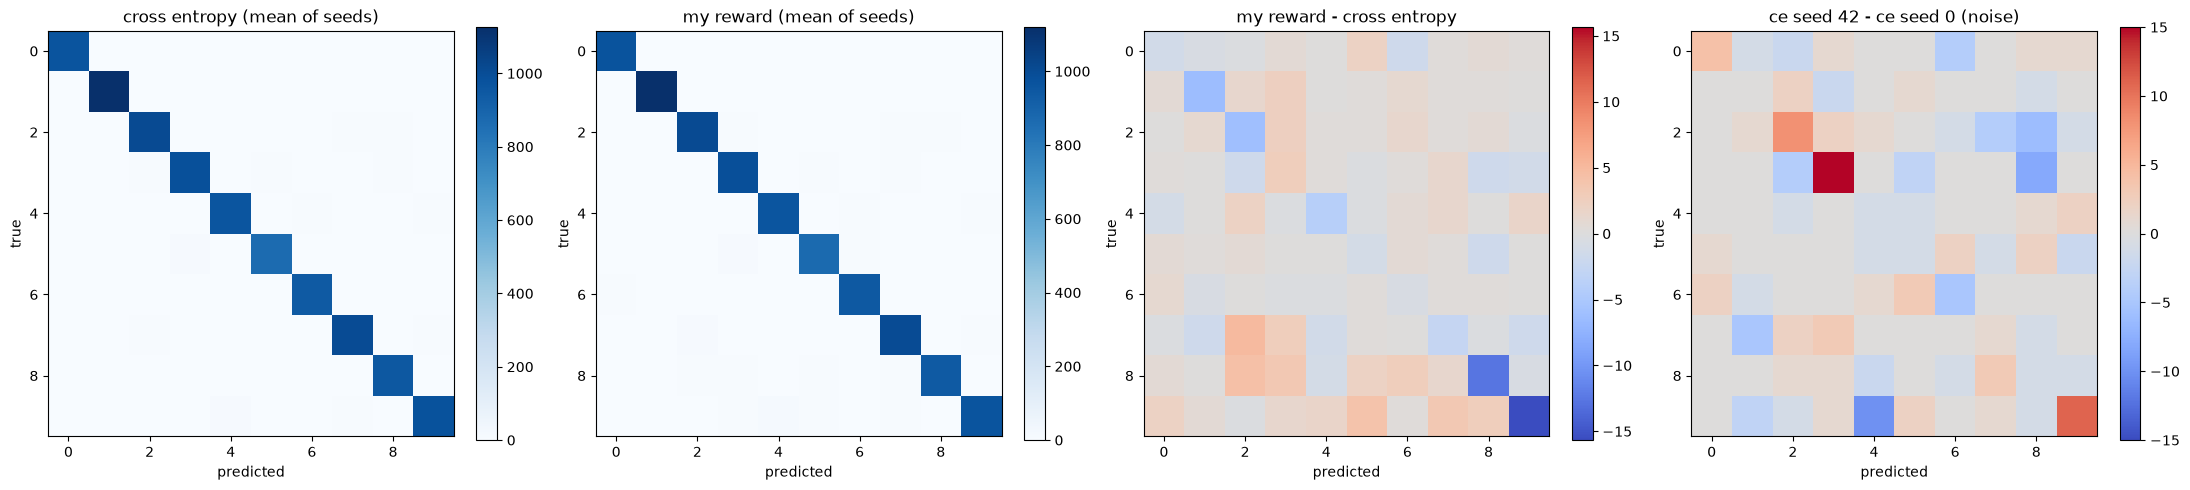
\includegraphics[width=0.98\textwidth]{fig_confusion_matrices.png}
\caption{Confusion matrices on the test set (mean over three seeds) for cross-entropy (left)
and the expected-cost criterion (second), their difference (third), and a seed-to-seed noise
baseline (right).}
\label{fig:cm}
\end{figure}

\section{Discussion}
\label{sec:disc}

\subsection{Loss versus Task Objective}
\label{sec:gap}

The two strictly proper rules behave differently from the rest. Squared error attains the
\textbf{lowest test cross-entropy ($0.0826 \pm 0.0007$)}, yet it is not the most accurate
($0.9785$); label smoothing attains the \textbf{highest accuracy ($0.9809 \pm 0.0009$)} but a
cross-entropy of $0.1558 \pm 0.0018$, nearly twice squared error's. The two quantities measure
different things: cross-entropy scores the whole probability vector and rewards calibrated
confidence, whereas accuracy scores only the $\arg\max$. One caution: label smoothing and
cross-entropy differ by only $0.0010$ in accuracy, with a standard error of the difference of
about $0.0009$, so the top two are \emph{not distinguishable}; only the direction is solid, not
a ranking. The robust statement is the negative one: the criterion with the lowest cross-entropy
is not the one with the highest accuracy, and the ranking on one metric does not transfer to the
other.

\subsection{Calibration}
\label{sec:cal}

Table~\ref{tab:cal} and Figure~\ref{fig:cal} report the expected calibration error (ECE) and
the mean confidence on the errors. For this model the result runs the opposite way to the usual
story: label smoothing has the highest accuracy but by far the \emph{worst} calibration
(ECE $0.089$, against $0.0135$ for cross-entropy and $0.0111$ for squared error). The mechanism
is simple and checkable rather than speculative: with $\epsilon=0.1$ over $K=10$ classes the
smoothed target for the true class is $1-\epsilon+\epsilon/K=0.91$, so the network is trained to
put about $0.91$ on the true class, while its accuracy is about $0.98$. The confidence is capped
below the accuracy almost by construction, which is exactly what an ECE with 15 bins measures;
the mean confidence on the errors is only $0.60$, against $0.85$ for cross-entropy. This is the
accuracy-versus-calibration trade-off made concrete. \textcite{muller2019} found
label smoothing usually \emph{improves} calibration on large networks; the cap argument shows why
the same mechanism can \emph{worsen} it when accuracy sits above the capped confidence, as it
does here, so the two results are consistent. Squared error, a proper rule, is the best
calibrated.

\begin{table}[htbp]
\centering
\small
\caption{Calibration on the test set (three-seed mean $\pm$ std), and the mean confidence on
the misclassified examples.}
\label{tab:cal}
\begin{tabular}{@{}lrr@{}}
\toprule
Criterion & Expected calibration error & Mean confidence on errors \\
\midrule
squared error & $0.0111 \pm 0.0004$ & 0.799 \\
cross-entropy & $0.0135 \pm 0.0007$ & 0.851 \\
absolute error & $0.0185 \pm 0.0004$ & 0.891 \\
expected cost (mine) & $0.0198 \pm 0.0001$ & 0.889 \\
label smoothing & $0.0890 \pm 0.0018$ & 0.596 \\
\bottomrule
\end{tabular}
\end{table}

\begin{figure}[htbp]
\centering
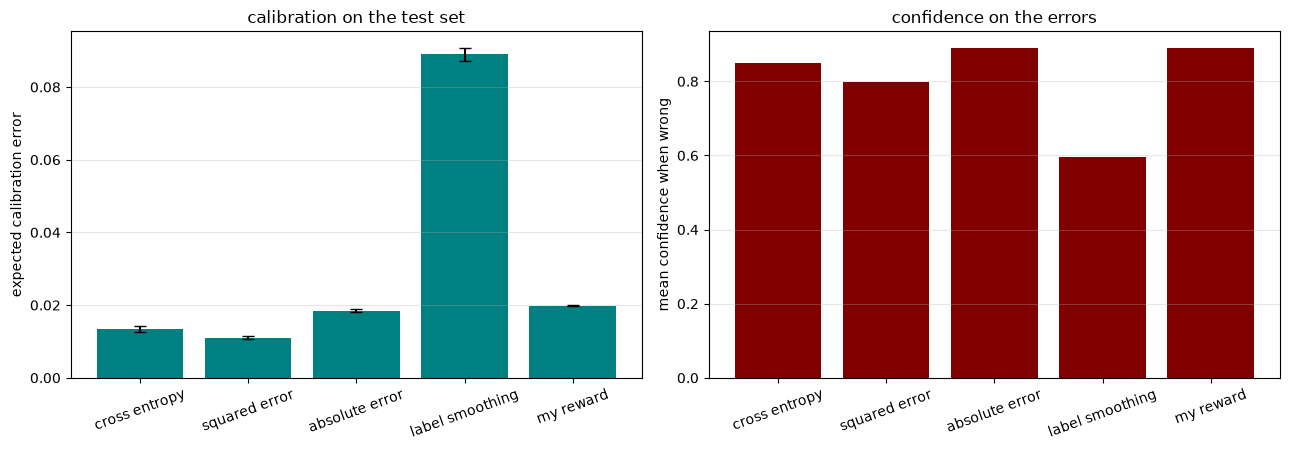
\includegraphics[width=0.9\textwidth]{fig_calibration.png}
\caption{Expected calibration error (left) and mean confidence on the errors (right), by
criterion.}
\label{fig:cal}
\end{figure}

\subsection{Why the Linear Criteria Fail}
\label{sec:linear}

Cross-entropy and label smoothing finish first and second on accuracy; the two improper,
\emph{linear} criteria finish last and second-last (expected cost $0.9751$, absolute error
$0.9766$). A likely reason is visible in the gradients. For squared error, absolute error and the
expected cost the logit gradient has the form
$\delta=\hat p\odot\big(g-\sum_j \hat p_j g_j\big)$, so every component carries a factor
$\hat p_k$; as the network becomes confidently wrong the gradient collapses toward zero, while
cross-entropy's $\delta=\hat p-y$ stays large (its true-class component is $-1$). Measuring the
per-example gradient norm on the misclassified test examples makes this concrete
(Figure~\ref{fig:grad}): cross-entropy $1.24$ and label smoothing $1.00$, against squared error
$0.19$, absolute error $0.15$, and the expected cost $0.058$. This is a \emph{correlation}, not a
controlled test: the gradient norm is measured on the trained models, and squared error shares
the same $\hat p\odot(\cdot)$ form and a gradient of only $0.19$ yet edges absolute error by just
$0.2$ points. The measurement is therefore \emph{consistent with} the vanishing-gradient
explanation, which is the most likely candidate, but it does not single it out as the cause. It
is still sharper than the earlier ``the minimiser is a corner'' description.

It also explains absolute error. For a softmax output inside $(0,1)$ and a one-hot target,
$\lVert\hat p-y\rVert_1=2(1-\hat p_y)$ is linear in $\hat p_y$, so absolute error is a linear
(improper) loss, in the same family as the hand-designed expected cost; the two linear losses
finish last and second-last, which is consistent with the gradient explanation. For the custom
criterion the dense reward matrix may compound the problem---the cost signal is small relative to
the pressure to be correct---and the gradient behaviour is the most plausible single explanation,
but the evidence here is correlational, so it is offered as such.

\begin{figure}[htbp]
\centering
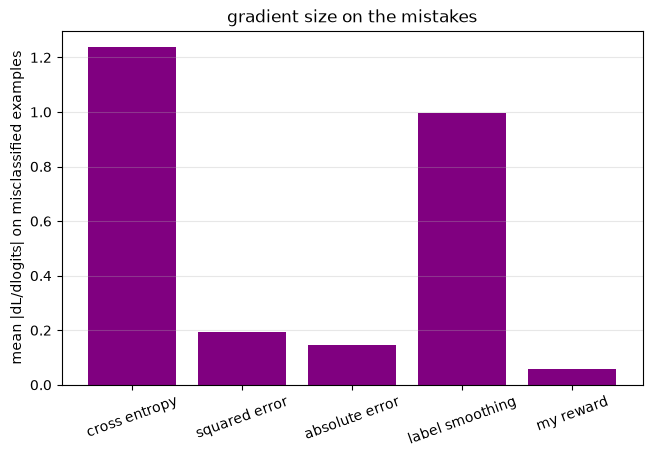
\includegraphics[width=0.6\textwidth]{fig_gradient_norms.png}
\caption{Mean per-example gradient magnitude on the misclassified test examples. The gradients
of the linear criteria vanish on the errors; cross-entropy's does not.}
\label{fig:grad}
\end{figure}

\subsection{Limitations}

(i) The reward matrix is a single hand-designed matrix; a different matrix, or one derived from
a baseline model's confusion matrix, could behave differently. (ii) The report does not include
a finite-difference verification of the analytic gradients; the backward pass was checked only
by the loss converging. (iii) The model is fixed at two $\tanh$ hidden layers, so the comparison
is specific to this architecture. (iv) Thirty epochs and three seeds are enough to separate the
large gaps but not the sub-0.1-point differences; the $0.0003$--$0.0013$ seed standard
deviations bound those, and there is no early stopping, so the test-cross-entropy ranking partly
reflects different overfitting (Section~\ref{sec:curves}). (v) The reward-over-errors and
fraction-similar metrics are weak: with a $2\%$ error rate and a dense matrix, the aggregate is
dominated by the diagonal and moves little, and the reward-over-errors gaps are within seed
noise. (vi) The calibration numbers are measured in-sample on the test set with 15 bins; a
deployment would fit the calibration on held-out data.

\subsection{Future Work}

The natural next step is to build the reward matrix from evidence rather than by hand: train a
baseline, read its confusion matrix, and set $R$ from the observed confusability. A second is to
replace the linear expected cost with a proper scoring rule on the designed target, which should
behave better than a gradient that vanishes on the mistakes. A third is to add a finite-difference
gradient check per criterion and early stopping, and to study the criterion on a task with a
genuinely asymmetric cost (for example, medical triage where one error type is far worse), where
the loss--objective gap is larger and the design decision matters more.

\section{Implementation Log}
\label{sec:log}

\subsection{Challenges and Solutions}

\paragraph{Gradients differ per criterion.} Almost all of the network is shared, but the logit
gradient $\delta^{(L)}$ changes with the criterion. Getting the softmax Jacobian right for
squared error and absolute error (the $\hat p_k(g_k-\sum_j\hat p_j g_j)$ form, rather than
simply $\hat p-y$) was the main derivation.

\paragraph{Numerical stability.} A naive softmax overflows for large logits, so the row maximum
is subtracted before exponentiating, and a small constant is added inside the logarithm so a
zero probability does not produce a \texttt{nan} from $0\cdot\log 0$.

\paragraph{Keeping the protocol honest.} An early version evaluated on the cross-validation
folds and labelled the plot ``test accuracy''. That is wrong: the folds are a validation set,
and any choice made while looking at them leaks. The final version reports cross-validation
separately and scores the test set once, after refitting on all the training data.

\paragraph{Corrections after review.} A first version of the results over-read the evidence in
three ways, each fixed here. The learning-curve figure plotted each criterion's own training loss
next to a cross-entropy validation curve, which is not comparable; both panels are now
cross-entropy. The confusion-matrix difference was quoted from a single seed (a largest cell of
$21$ counts) with no baseline; it is now the seed average, and a seed-to-seed baseline shows the
difference ($15.7$, seed-averaged) is the same size as the single-seed noise ($15.0$), so the
confusion result is not significant. And the calibration claim was asserted without measurement;
ECE and the confidence on the errors are now reported. Recording these is part of the work.

\paragraph{Scope control.} An earlier draft also included a label-noise experiment and a
sigmoid-versus-squared-error study. Both were dropped to keep the project on one thread: the
comparison of training criteria.

\subsection{Use of AI Tools}

AI assistance was used to scaffold parts of the code and to help draft and edit this report. The
critical-thinking steps were kept by the author: the criteria and their gradients, the reward
matrix, and the interpretation of the negative result for the custom criterion. An earlier
convolutional extension suggested by the assistant was removed because it could not be defended
under questioning. Every measured number reported here is written to \texttt{metrics.json} by
the notebook; the parameter count and the reported differences are arithmetic on those outputs.

\subsection{Knowledge Gaps}

\paragraph{Why cross-entropy is preferred.} The support for cross-entropy is the derivation, not
the measured ranking. It is the negative log-likelihood for a categorical target, a strictly
proper scoring rule, and its logit gradient $(\hat p-y)$ does not vanish when the model is
confidently wrong. The measured accuracies do not by themselves establish a preference: label
smoothing is statistically indistinguishable from it on accuracy, and its reward-over-errors lead
is within seed noise. The argument rests on the derivation and on the gradient behaviour
(Section~\ref{sec:linear}); the gradient-norm measurement is consistent with it, though it is
correlational rather than a controlled test.

\paragraph{Why the custom criterion underperformed.} This was initially surprising. Writing the
expected cost as $\sum_k\hat p_k c_k$ shows it is linear in the probabilities, so it is not a
proper scoring rule and---more precisely than ``its optimum is a corner''---its logit gradient
carries a factor of the predicted probability and vanishes on the confidently-wrong examples it
should be correcting. The gradient-norm measurement (Section~\ref{sec:linear}) is consistent with
this, though it is a correlation on the trained model rather than a controlled test.

\section{Conclusion}

A multi-layer perceptron was implemented from scratch in NumPy and studied through its training
criterion. The choice of criterion matters: accuracy ranges from $0.9751$ to $0.9809$ across
five criteria trained identically. The two improper, \emph{linear} criteria (absolute error and
the hand-designed expected cost) finish last and second-last, and measuring the per-example
gradient norm on the mistakes is consistent with the explanation that their gradients carry a
factor of the predicted probability and vanish when the model is confidently wrong, while
cross-entropy's does not (correlational, not a controlled test). The
results also show a clear loss--objective gap: the criterion with the lowest test cross-entropy
(squared error) is not the most accurate, and the most accurate criterion (label smoothing) is
the worst calibrated. Designing a cost can express a preference, but it does not by itself
produce a better model.

\printbibliography

\end{document}
